\chapter{State of the art}

\section{Intraoperative ultrasound}
\textcolor{red}{Start with why US is used, then describe how it works and the limitations. from there you should have a nice transition to navigation}
Ultrasound imaging works by the \textit{pulse-echo} principle. A short
ultrasound-pulse is emitted from a transducer. Then the soundwaves get
transmitted and reflected differently by different tissues. The reflected
soundwaves travel back into the transducer and get converted into an electrical
signal. After post-processing these signals become ultrasound images. Basically
the ultrasound measures the mechanical properties of the tissue. The tissues
have different acoustic impedance, which is the product of tissue density and
ultrasound speed in travelling through the tissue. The resolution of the
ultrasound images depends on the frequency of the ultrasound waves. High
frequencies lead to high resolutions but low depth into the tissue because the
absorption of the sound energy increases with frequency too. Therefore the
useability to see deep structures is limited \cite{torzilli2014ultrasound}. In
liver surgeries the ultrasound is used for intraoperative planning and
navigation inside the liver. Figure \ref{fig:liverUS} shows an example of an
ultrasound image of the liver and its corresponding position in the 3D liver
model. The surgeon can find the tumors inside the liver by using the ultrasound.
Registration methods based on 3D ultrasound reconstructed liver vessels also
exist but are not used in practice a lot yet \cite{lange2003vessel}. Therefore
ultrasound is an important and established instrument in liver surgeries.

\begin{figure}[H]
  \centering
 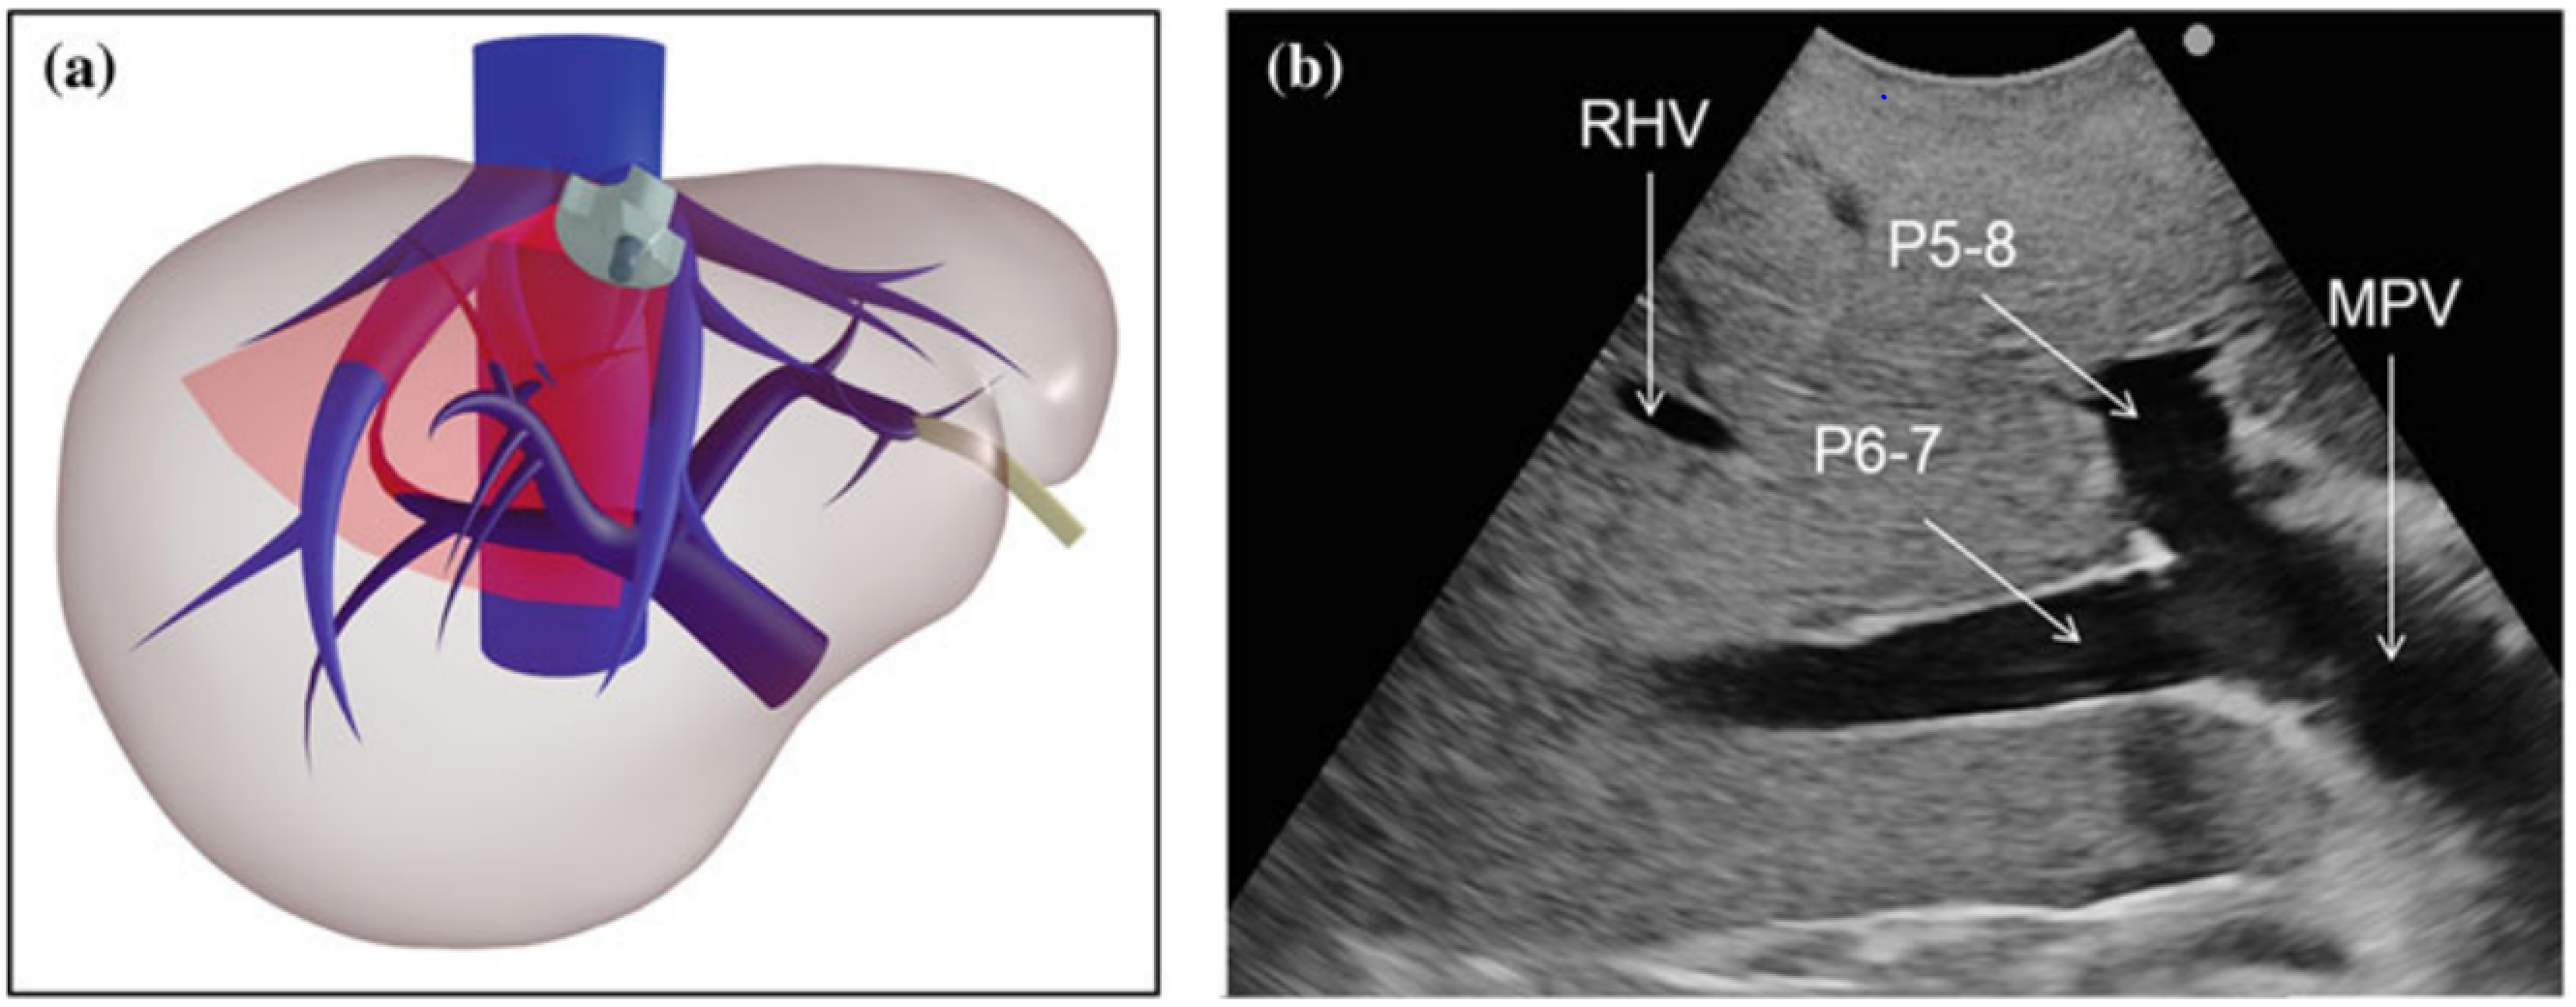
\includegraphics[width=\textwidth]{liverUS}
 \caption{ Left (a) ultrasound image plane in the liver. Right (b) intraoperative
   ultrasound image. One can see the right hepatic vein (RHV), the portal branch
   to segments 5 and 8 (P5-8) and the portal branch to segments 6 and 7 (P6-7) \cite{torzilli2014ultrasound}}
  \label{fig:liverUS}
\end{figure}

\section{Navigation for liver resections}
\textcolor{red}{first, why is navigation needed, then how does it generally work 1) preoperative model or surgical plan 2) tracking 3) registration 4) navigation visualization etc. then challenges especially in liver surgery and limitations}
The actual intervention in computer assisted surgeries (CAS) is defined as
surgical navigation. For navigated surgeries special instruments are used. These
instruments are tracked by the naviagation system. The orientation and position
of the instruments in relation to the patient's anatomy is visualized on a
monitor in the operating room. The surgeon can then see what he does on the
monitor and uses the system to navigate the location and position of its
instruments. This is specialy then useful when the tip of the instrument is not
actually visible for the suergeon. 
In liver surgeries, the navigation is mostly done by first registering the patient to a pre-operative 3D
computer tomography (CT) scan of the liver during the surgery. All surgical
instruments have trackable markers attached to them and a tracking camera sees
these markers and can differentiate the different instruments from their attached
markers. The achieved
navigation accuracy with such a system was 4.5 mm $\pm$3.6 mm averaged over nine surgeries \cite{peterhans2011navigation}.
Current research tries to compensate for deformations of the liver after the CT
scan to the actual shape of the liver \cite{clements2017deformation}
\cite{clements2015validation}. 
\subsection{Creation of preoperative 3D-models}


\cite{numminen2005preoperative} time consuming and method to create 3d-model
from CT

\subsection{Registration methods}
Different registration methods exist. Discrete landmarks, surface scans and
volumetric sonography scans are just a few of the approaches that can be
used to achieve precise alignment of the preoperative image data with the
surgical site \cite{banz2016intraoperative}.

\subsection{Tracking modalities}
To track surgical instruments and patient's anatomy (define the position and
orientation in real time) during naviagated surgery a tracking system is needed.
Tracking can be done by different technologies. The most used tracking
modality is optical tracking. 

\subsubsection{Optical tracking}
Optical tracking is the most used tracking modality in naviagated liver
surgeries. Passive markers (spherical, retro-reflective that reflect infrared
light) or active markers (infrared-emitting markers that are activated by an
electrical signal) \cite{wiles2004accuracy} are attached to the objects that
need to be tracked. A tracking camera is then emitting infrared light by illuminators
on the position sensor (only for passive markers). The position sensor
determines the position and orientation of the tracked instruments based on the
information it receives from those markers \cite{noauthor_polaris_nodate}.  

\section{Surface reconstruction of unorganized points}
\textcolor{red}{First, collecting the sample ... These terms should match the titles below
Both other chapters, explain first what the process is for, then what methods are available}
A surface reconstruction's goal is to create a surface from sampling points. Two
main steps need to be processed. First, collecting the sample points. Second,
apply a reconstruction algorithm to the sampled points.
\subsection{Data acquisition}
There exist different methods of collecting surface points
\cite{franca20053d}\cite{levoy2000digital}\cite{cui20113d}\cite{chu2002infrared}\cite{dou20153d}.
Optical (non-contact scan) scans are the most popular ones. Specialy laser based
scanners can scan very fast and with a precision in the order of micrometers. Also contact scans exist
\cite{pai2001scanning}. Contact scans can also be very precise (in the order of
micrometers).
Only a few articles were published in the field of liver surface scanning \cite{maier2014comparative} \cite{thompson2015accuracy}. 
They used stereo laparoscopic cameras to sample the surface.
The resulting sampling points lie on or near an unknown surface. A
reconstruction algorithm has now to reconstruct the surface from these points.
\subsection{Reconstruction algorithms}
\textcolor{red}{ switch explicit and implicit, so you have the same order as in the figure}
Again, a lot of reconstruction algorithms exist \cite{lim2014surface}, but not
all of them are made to reconstruct from unorganized points. This means
that the point orders, orientations, connections and the topological type of the
surface is not known a priori. Therefore it is necessary that the algorithm does not assume any structure
on the data points \cite{hornung2006robust} \cite{yu1999surface}. The orientations, connections and the topological
type must be inferred from the points. This is a major difficulty of the general surface
reconstruction problem \cite{hoppe1992surface}. In the past few decades, many
algorithms that can solve this problem have been published. Nevertheless it is
still a challanging task that is part of current research \cite{li2018surface}.
The available reconstrction types can be classified into two groups: implicit
volume-based and explicit mesh-based reconstructions.
\begin{figure}[H]
  \centering
 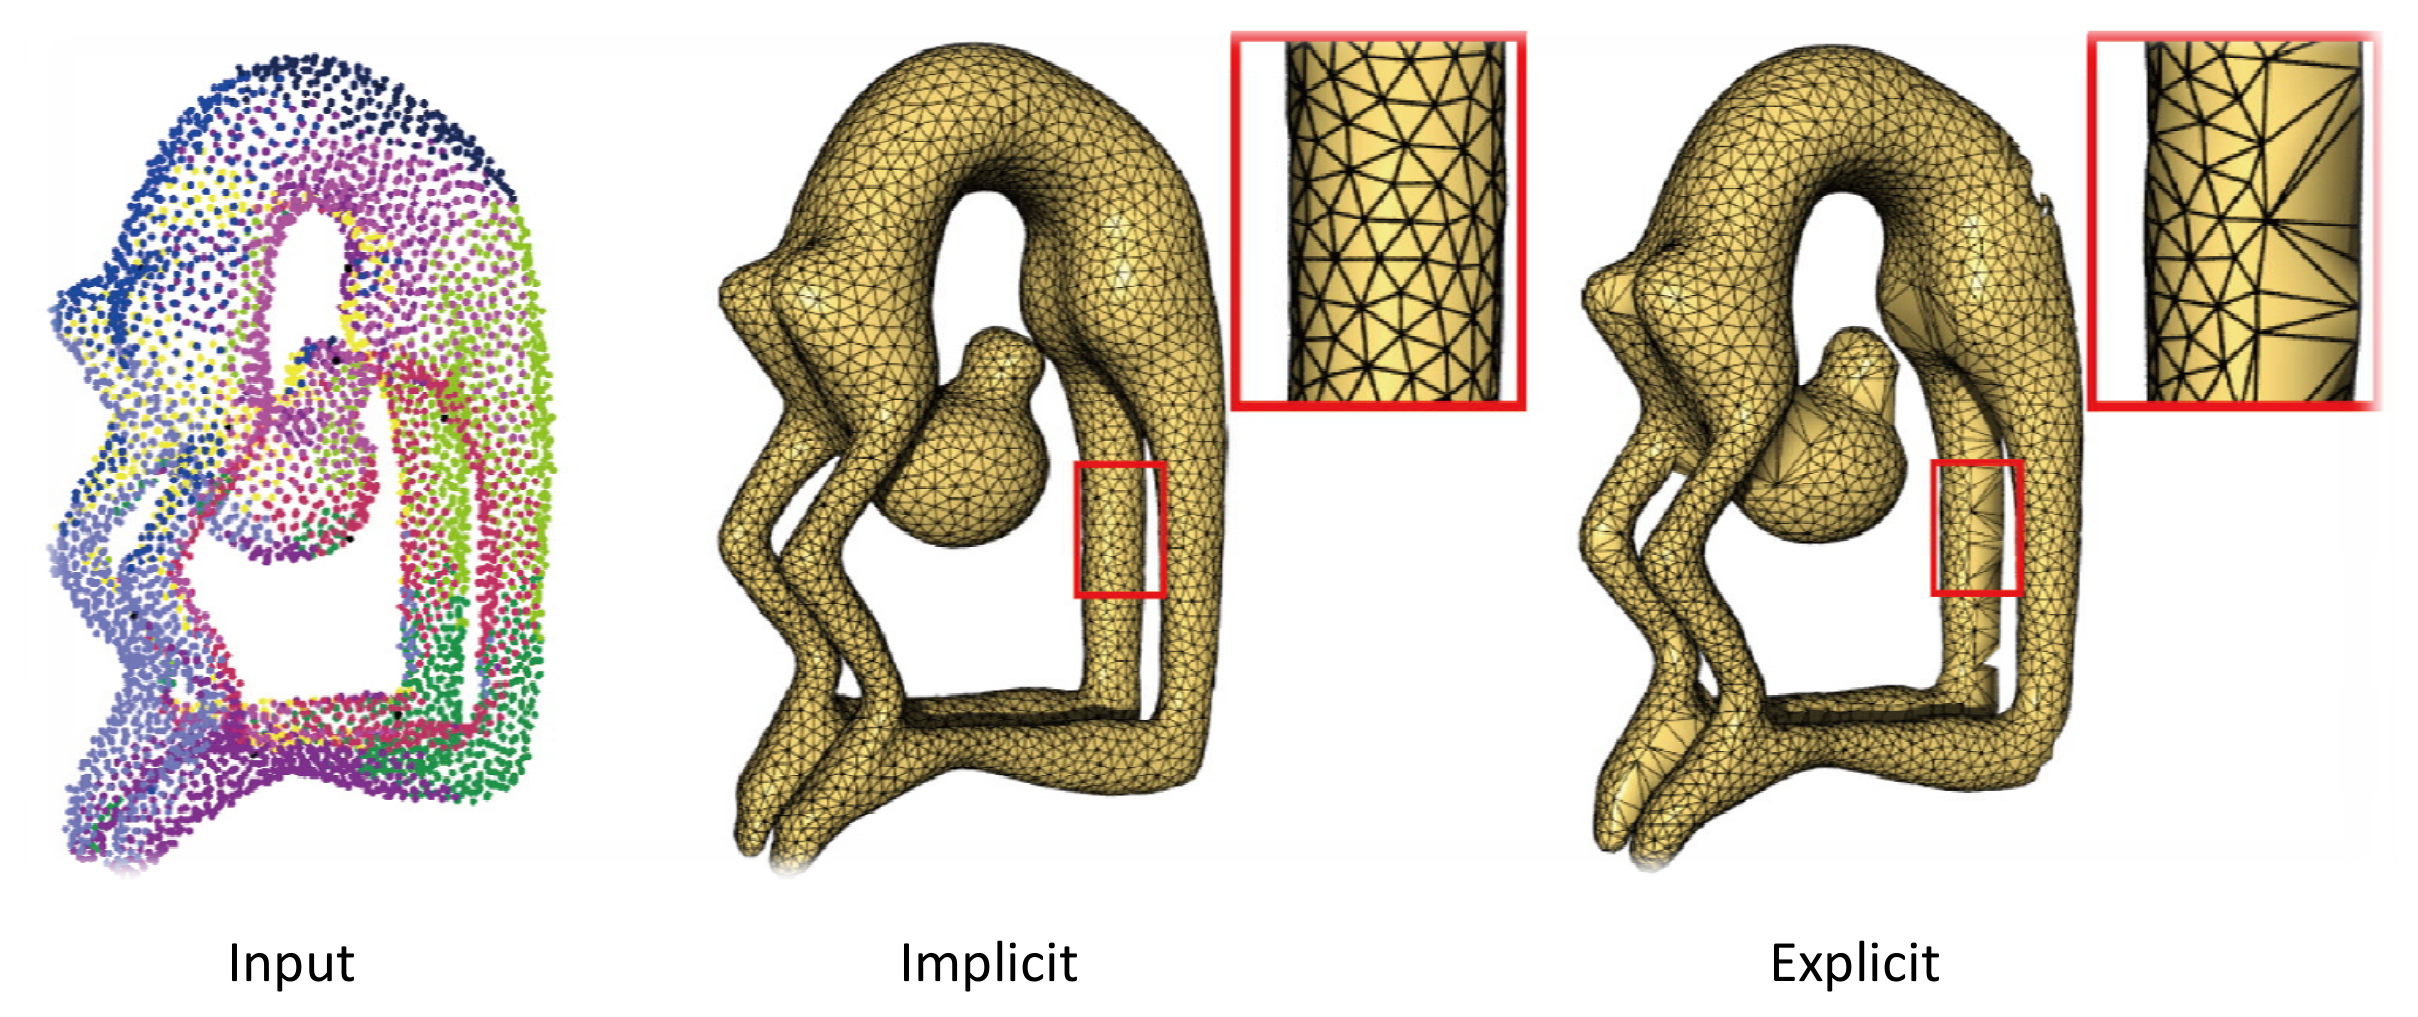
\includegraphics[width=\textwidth]{ImplicitVSExplicit}
 \caption{The difference between implicit and explicit surface reconstructions.
   On the left side is the pointcloud used as input. In the middle the result of an
   implicit reconstruction. On the right side the result of an explicit
   reconstruction \cite{stanfordPP}}
  \label{fig:ImplicitVSExplicit}
\end{figure}
\subsubsection{Explicit mesh-based reconstrction}
Explicit mesh-based reconstrction methods form a triangular mesh directly from
the unorganized points. These mesh-based reconstructions are precise but they
have problems with noise, complex shapes and especially holes in data.
\subsubsection{Implicit volume-based reconstrction}
Implicit volume-based reconstruction techniques construct an implicit
volume-function from the input points. From the iso-surface of the
volume-function a restored surface can then be optained. For these methods it is
not a problem if the surface topology is complex. But most of these methods
suffer from oversmoothing the data and the need of accurate directions of normal
vectors in addition to the unorganized points. 


\cite{kazhdan2005reconstruction} oriented point set hornung2006robust
\cite{hornung2006robust} non uniformly sampled point clouds without normal information
\cite{yu1999surface} NN to reconstruct from unorganized points



% \begin{itemize}
%   \item not tracked laproscopic one shot images stereo with registration
%   \item moved laproscopic tracked endoscope stereo with registration 
% \end{list}

% \cite{hoppe1992surface}

\endinput
%%% Local Variables:
%%% TeX-master: "MscThesis"
%%% End: